\hrule
\begin{center}
{\large\bf Lernaufgaben zur Klausur 2}\\[-0mm]
Studienkolleg der TU Berlin\hfill Till Zoppke\\
Informatik Oberkurs \hfill \today
\end{center}
\hrule

\section*{Aufgabe 1: Klassische KI und maschinelles Lernen}

\noindent Erklären Sie den Unterschied zwischen klassischer KI und
maschinellem Lernen.

\loesung{
  Bei der \textbf{klassischen KI} liegt die Intelligenz beim Menschen. Er oder sie entwickelt eine Strategie für die Lösung des Problems und setzt diese als Computerprogramm um. Das System verhält sich nach den Regeln, die die Entwickler:innen programmiert haben.

  Beim \textbf{maschinellen Lernen} liegt die Intelligenz beim Computersystem. Die Entwickler:innen definieren das Problem und programmieren das Computersystem so, dass es die Lösungsstrategie anhand von Trainingsdaten selbst lernt.
}

\section*{Aufgabe 2: Umgebungsvariablen}

\noindent Umgebungsvariablen werden in Linux z.\,B. dafür genutzt, einen
API-Key außerhalb des Programmcodes zu speichern.

\begin{enumerate}[label=\alph*)]
\item Mit welchem Kommando wird in der \texttt{bash} eine Umgebungsvariable gesetzt?
\loesung{\texttt{export VARIABLENNAME=wert} \quad
  Beispiel: \texttt{export CHATAI\_API\_KEY=mein\_schluessel}}

\item Mit welchem Kommando kann ihr Wert im Terminal ausgegeben werden?
\loesung{\texttt{echo \$VARIABLENNAME} \quad
  Beispiel: \texttt{echo \$CHATAI\_API\_KEY}}

\item Welchen Nutzen hat es, einen API-Key in einer Umgebungsvariablen
abzulegen, statt ihn direkt im Programmcode zu schreiben?
\loesung{
  Der API-Key steht nicht im Quellcode. Das Programm kann also geteilt werden, ohne dass der Schlüssel kompromittiert wird. Außerdem kann der Schlüssel geändert werden, ohne den Code zu bearbeiten, und verschiedene Nutzer können eigene Schlüssel verwenden.
}
\end{enumerate}

\section*{Aufgabe 3: Dictionaries}

\noindent \textbf{a)} Schreiben Sie an jede leere Stelle, was die Python-Konsole hier ausgeben würde.

\begin{lstlisting}[style=python]
>>> staedte = {"Berlin": "im Sommer", "Hamburg": "schoen"}
>>> staedte["Hamburg"]
(*@\ifdefined\zeigloesungen\textcolor{loesgruen}{'schoen'}\else\antwortmarker\fi@*)
>>> "Muenchen" in staedte
(*@\ifdefined\zeigloesungen\textcolor{loesgruen}{False}\else\antwortmarker\fi@*)
>>> staedte["Muenchen"] = "auch schoen"
>>> len(staedte)
(*@\ifdefined\zeigloesungen\textcolor{loesgruen}{3}\else\antwortmarker\fi@*)
\end{lstlisting}

\medskip
\noindent \textbf{b)} Bearbeiten Sie die folgenden Fragen zum Dictionary \texttt{tiere} und geben Sie den jeweiligen Python-Code an.

\begin{lstlisting}[style=python]
tiere = {
    "Flipper": {
        "tierart": "Delphin",
        "klasse": "Saeugetier",
        "futter": ["Hering", "Makrele", "Schokolade"],
        "merkmale": {
            "koerperlaenge": {"wert": 2.5, "einheit": "m"},
        },
    },
    "Goldi": {
        "tierart": "Guppy",
        "klasse": None,
    },
}
\end{lstlisting}

\begin{enumerate}[label=\alph*)]
\item Wie erhält man die Tierart von Flipper?\\
\ifdefined\zeigloesungen\texttt{\textcolor{loesgruen}{tiere[\dq Flipper\dq][\dq tierart\dq]}}\fi

\item Wie erhält man die Zahl $2{,}5$ als Körperlänge von Flipper?\\
\ifdefined\zeigloesungen\texttt{\textcolor{loesgruen}{tiere[\dq Flipper\dq][\dq merkmale\dq][\dq koerperlaenge\dq][\dq wert\dq]}}\fi

\item Wie setzt man bei Flipper das Merkmal \lstinline|"beine"| mit Wert 0 und Einheit \lstinline|"Anzahl"|?\\
\ifdefined\zeigloesungen\texttt{\textcolor{loesgruen}{tiere[\dq Flipper\dq][\dq merkmale\dq][\dq beine\dq] = \{\dq wert\dq: 0, \dq einheit\dq: \dq Anzahl\dq\}}}\fi

\item Wie entfernt man \lstinline|"Schokolade"| aus der Futterliste von Flipper?\\
\ifdefined\zeigloesungen\texttt{\textcolor{loesgruen}{tiere[\dq Flipper\dq][\dq futter\dq].remove(\dq Schokolade\dq)}}\fi

\item Wie setzt man die Klasse von Goldi auf \lstinline|"Fisch"|?\\
\ifdefined\zeigloesungen\texttt{\textcolor{loesgruen}{tiere[\dq Goldi\dq][\dq klasse\dq] = \dq Fisch\dq}}\fi
\end{enumerate}

\section*{Aufgabe 4: Perzeptron-Lernalgorithmus nachvollziehen}

\noindent Ein Perzeptron soll Tiere anhand von zwei Merkmalen klassifizieren: $x_1$ ist die Anzahl der Beine, $x_2$ ist die Körperlänge in Metern. Verwenden Sie die Kodierung $+1 = \text{Säugetier}$ und $-1 = \text{Fisch}$. Gegeben sind die folgenden Trainingsdaten:
\begin{center}
\begin{tabular}{|l|>{\centering\arraybackslash}p{2.2cm}|>{\centering\arraybackslash}p{2.8cm}|>{\centering\arraybackslash}p{2.2cm}|}
\hline
\textbf{Tier} & \textbf{Beine $x_1$} & \textbf{Länge $x_2$} & \textbf{Klasse $y$} \\
\hline
Delphin & 0 & $2{,}5$ & $+1$ \\
\hline
Forelle & 0 & $0{,}4$ & $-1$ \\
\hline
Guppy & 0 & $0{,}05$ & $-1$ \\
\hline
Hausmaus & 4 & $0{,}08$ & $+1$ \\
\hline
Känguru & 2 & $1{,}6$ & $+1$ \\
\hline
\end{tabular}
\end{center}
\medskip

\noindent \textbf{a)} Tragen Sie die Trainingsdaten in das Diagramm ein. Markieren Sie Säugetiere mit einem \textbf{x} und Fische mit einem \textbf{o}.

\begin{center}
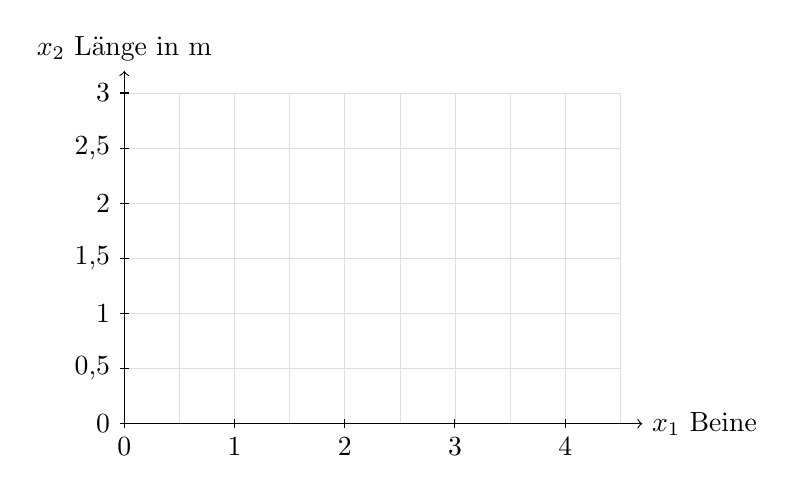
\begin{tikzpicture}[x=1.4cm,y=1.4cm]
\draw[step=0.5,gray!25,very thin] (0,0) grid (4.5,3);
\draw[->] (0,0) -- (4.7,0) node[right] {$x_1$ Beine};
\draw[->] (0,0) -- (0,3.2) node[above] {$x_2$ Länge in m};
\foreach \x in {0,1,2,3,4}
    \draw (\x,0.04) -- (\x,-0.04) node[below] {\x};
\foreach \y/\label in {0/0,0.5/0{,}5,1/1,1.5/1{,}5,2/2,2.5/2{,}5,3/3}
    \draw (0.04,\y) -- (-0.04,\y) node[left] {\label};
\ifdefined\zeigloesungen
  % Säugetiere: x
  \node[font=\bfseries,text=loesgruen] at (0,2.5)   {x}; % Delphin
  \node[font=\bfseries,text=loesgruen] at (4,0.08)  {x}; % Hausmaus
  \node[font=\bfseries,text=loesgruen] at (2,1.6)   {x}; % Känguru
  % Fische: o
  \node[font=\bfseries,text=loesgruen] at (0,0.4)   {o}; % Forelle
  \node[font=\bfseries,text=loesgruen] at (0,0.05)  {o}; % Guppy
  % Trenngerade: -1 + 4*x1 + 1.73*x2 = 0  =>  x2 = (1 - 4*x1) / 1.73
  % x1=0 => x2=0.578;  x1=0.25 => x2=0
  \draw[loesgruen,thick] (0,0.578) -- (0.25,0);
\fi
\end{tikzpicture}
\end{center}

\noindent \textbf{b)} Führen Sie den Algorithmus für zwei Epochen per Hand durch. Tragen Sie in jeder Zeile die Werte ein, die der Algorithmus für die entsprechende Eingabe berechnet. Notieren Sie bei Updates explizit, wie die Gewichte angepasst werden. Prüfen Sie anschließend, ob der Algorithmus nach diesen zwei Epochen bereits konvergiert ist.

\begin{tcolorbox}[title=Der Perzeptron-Lernalgorithmus (Pseudocode)]
\begin{tabbing}
\hspace{1.5em}\=\hspace{1.5em}\=\hspace{1.5em}\=\kill
\textbf{Trainingsdaten:} Beispiele $(x_1^{(k)}, x_2^{(k)}, y^{(k)})$ für $k = 1, \ldots, m$ mit $y^{(k)} \in \{-1, +1\}$\\[1mm]
\textbf{Initialisierung:} $w_0 = 0$, $w_1 = 0$, $w_2 = 0$\\[1mm]
\textbf{Wiederhole}, bis eine Epoche komplett fehlerfrei durchlaufen wird:\\[1mm]
\>\textbf{Für jedes} Trainingsbeispiel $(x_1, x_2, y)$:\\[1mm]
\>\>Berechne $z = w_0 + w_1 x_1 + w_2 x_2$ und $\hat{y} = \operatorname{sign}(z)$\\[1mm]
\>\>\textbf{Falls} $\hat{y} \neq y$: \quad \pseudocomment{Fehlklassifikation}\\[1mm]
\>\>\>$w_0 \leftarrow w_0 + y$; \quad $w_1 \leftarrow w_1 + y \cdot x_1$; \quad $w_2 \leftarrow w_2 + y \cdot x_2$\\[1mm]
\textbf{Ausgabe:} Gewichte $w_0, w_1, w_2$, die alle Trainingsbeispiele korrekt klassifizieren.
\end{tabbing}
\end{tcolorbox}
\medskip

\noindent\begin{tabular}{@{}p{.8cm}@{}l@{}}
\hspace{-0.5cm}\tiny{Epoche 1} &
\begin{tabular}{|>{\centering\arraybackslash}p{1.7cm}|>{\centering\arraybackslash}p{0.8cm}|p{6cm}|>{\centering\arraybackslash}p{0.8cm}|>{\centering\arraybackslash}p{1.2cm}|>{\centering\arraybackslash}p{2.4cm}|}
\hline
Tier & $y$ & Berechnung z & $\hat y$ & \small{Fehler?} & \small{neue Gewichte} \\
\hline
Start & -- & -- & -- & -- & $(0; 0; 0)$ \\
\hline
\textcolor{blue}{Delphin} & \textcolor{blue}{$+1$} & \textcolor{blue}{$z = 0 + 0\cdot0 + 0\cdot2{,}5 = 0$} & \textcolor{blue}{$0$} & \textcolor{blue}{ja} & \textcolor{blue}{$(1;0;2{,}5)$} \\[8pt]
\hline
Forelle & \ifdefined\zeigloesungen \textcolor{loesgruen}{$-1$} \else $-1$ \fi & \ifdefined\zeigloesungen \textcolor{loesgruen}{$z = 1 + 0\cdot0 + 2{,}5\cdot0{,}4 = 2$} \fi & \ifdefined\zeigloesungen \textcolor{loesgruen}{$+1$} \fi & \ifdefined\zeigloesungen \textcolor{loesgruen}{ja} \fi & \ifdefined\zeigloesungen \textcolor{loesgruen}{$(0;0;2{,}1)$} \fi \\[8pt]
\hline
Guppy & \ifdefined\zeigloesungen \textcolor{loesgruen}{$-1$} \else $-1$ \fi & \ifdefined\zeigloesungen \textcolor{loesgruen}{$z = 0 + 0\cdot0 + 2{,}1\cdot0{,}05 \approx 0{,}11$} \fi & \ifdefined\zeigloesungen \textcolor{loesgruen}{$+1$} \fi & \ifdefined\zeigloesungen \textcolor{loesgruen}{ja} \fi & \ifdefined\zeigloesungen \textcolor{loesgruen}{$(-1;0;2{,}05)$} \fi \\[8pt]
\hline
Hausmaus & \ifdefined\zeigloesungen \textcolor{loesgruen}{$+1$} \else $+1$ \fi & \ifdefined\zeigloesungen \textcolor{loesgruen}{$z = {-1} + 0\cdot4 + 2{,}05\cdot0{,}08 \approx {-0{,}84}$} \fi & \ifdefined\zeigloesungen \textcolor{loesgruen}{$-1$} \fi & \ifdefined\zeigloesungen \textcolor{loesgruen}{ja} \fi & \ifdefined\zeigloesungen \textcolor{loesgruen}{$(0;4;2{,}13)$} \fi \\[8pt]
\hline
Känguru & \ifdefined\zeigloesungen \textcolor{loesgruen}{$+1$} \else $+1$ \fi & \ifdefined\zeigloesungen \textcolor{loesgruen}{$z = 0 + 4\cdot2 + 2{,}13\cdot1{,}6 \approx 11{,}41$} \fi & \ifdefined\zeigloesungen \textcolor{loesgruen}{$+1$} \fi & \ifdefined\zeigloesungen \textcolor{loesgruen}{nein} \fi & \ifdefined\zeigloesungen \textcolor{loesgruen}{$(0;4;2{,}13)$} \fi \\[8pt]
\hline
\end{tabular}
\end{tabular}
\medskip

\noindent\begin{tabular}{@{}p{.8cm}@{}l@{}}
\hspace{-0.5cm}\tiny{Epoche 2} &
\begin{tabular}{|>{\centering\arraybackslash}p{1.7cm}|>{\centering\arraybackslash}p{0.8cm}|p{6cm}|>{\centering\arraybackslash}p{0.8cm}|>{\centering\arraybackslash}p{1.2cm}|>{\centering\arraybackslash}p{2.4cm}|}
\hline
Tier & $y$ & Berechnung z & $\hat y$ & \small{Fehler?} & \small{neue Gewichte} \\
\hline
Delphin & \ifdefined\zeigloesungen \textcolor{loesgruen}{$+1$} \else $+1$ \fi & \ifdefined\zeigloesungen \textcolor{loesgruen}{$z = 0 + 4\cdot0 + 2{,}13\cdot2{,}5 \approx 5{,}33$} \fi & \ifdefined\zeigloesungen \textcolor{loesgruen}{$+1$} \fi & \ifdefined\zeigloesungen \textcolor{loesgruen}{nein} \fi & \ifdefined\zeigloesungen \textcolor{loesgruen}{$(0;4;2{,}13)$} \fi \\[8pt]
\hline
Forelle & \ifdefined\zeigloesungen \textcolor{loesgruen}{$-1$} \else $-1$ \fi & \ifdefined\zeigloesungen \textcolor{loesgruen}{$z = 0 + 4\cdot0 + 2{,}13\cdot0{,}4 \approx 0{,}85$} \fi & \ifdefined\zeigloesungen \textcolor{loesgruen}{$+1$} \fi & \ifdefined\zeigloesungen \textcolor{loesgruen}{ja} \fi & \ifdefined\zeigloesungen \textcolor{loesgruen}{$(-1;4;1{,}73)$} \fi \\[8pt]
\hline
Guppy & \ifdefined\zeigloesungen \textcolor{loesgruen}{$-1$} \else $-1$ \fi & \ifdefined\zeigloesungen \textcolor{loesgruen}{$z = {-1} + 4\cdot0 + 1{,}73\cdot0{,}05 \approx {-0{,}91}$} \fi & \ifdefined\zeigloesungen \textcolor{loesgruen}{$-1$} \fi & \ifdefined\zeigloesungen \textcolor{loesgruen}{nein} \fi & \ifdefined\zeigloesungen \textcolor{loesgruen}{$(-1;4;1{,}73)$} \fi \\[8pt]
\hline
Hausmaus & \ifdefined\zeigloesungen \textcolor{loesgruen}{$+1$} \else $+1$ \fi & \ifdefined\zeigloesungen \textcolor{loesgruen}{$z = {-1} + 4\cdot4 + 1{,}73\cdot0{,}08 \approx 15{,}14$} \fi & \ifdefined\zeigloesungen \textcolor{loesgruen}{$+1$} \fi & \ifdefined\zeigloesungen \textcolor{loesgruen}{nein} \fi & \ifdefined\zeigloesungen \textcolor{loesgruen}{$(-1;4;1{,}73)$} \fi \\[8pt]
\hline
Känguru & \ifdefined\zeigloesungen \textcolor{loesgruen}{$+1$} \else $+1$ \fi & \ifdefined\zeigloesungen \textcolor{loesgruen}{$z = {-1} + 4\cdot2 + 1{,}73\cdot1{,}6 \approx 9{,}77$} \fi & \ifdefined\zeigloesungen \textcolor{loesgruen}{$+1$} \fi & \ifdefined\zeigloesungen \textcolor{loesgruen}{nein} \fi & \ifdefined\zeigloesungen \textcolor{loesgruen}{$(-1;4;1{,}73)$} \fi \\[8pt]
\hline
\end{tabular}
\end{tabular}
\medskip

\noindent\antwortmarker \textbf{Gewichte nach zwei Epochen:}
$w_0 = \ifdefined\zeigloesungen \textcolor{loesgruen}{\mathbf{-1}} \else \gewichtsbox \fi$, \quad
$w_1 = \ifdefined\zeigloesungen \textcolor{loesgruen}{\mathbf{4}} \else \gewichtsbox \fi$, \quad
$w_2 = \ifdefined\zeigloesungen \textcolor{loesgruen}{\mathbf{1{,}73}} \else \gewichtsbox \fi$

\noindent Konvergiert nach zwei Epochen? \quad
\ifdefined\zeigloesungen
  $\Box$ ja \quad \textcolor{loesgruen}{$\boxtimes$ nein}
  \quad\textcolor{loesgruen}{\textit{(Epoche~2 enthielt noch einen Fehler bei der Forelle.)}}
\else
  $\Box$ ja \quad $\Box$ nein
\fi
\bigskip

\noindent \textbf{c)} Zeichnen Sie die Trenngerade zu den Gewichten nach zwei Epochen in das Diagramm ein. Hinweis: sie erhalten die Geradengleichung, indem sie $w_0 + w_1 x_1 + w_2 x_2 = 0$ setzen.

\loesung{
  Mit $w_0 = -1$, $w_1 = 4$, $w_2 = 1{,}73$ ergibt sich:
  \[
    -1 + 4x_1 + 1{,}73\, x_2 = 0
    \;\Longrightarrow\;
    x_2 = -\frac{4}{1{,}73}\, x_1 + \frac{1}{1{,}73}
    \;\approx\;
    -2{,}31\, x_1 + 0{,}58
  \]
}
\medskip

\noindent \textbf{d)} Ihr Perzeptron hat gelernt, Tier zu klassifizieren. Überprüfen Sie den Klassifikator mit den folgenden Eingaben und füllen Sie die leeren Felder aus.

\begin{center}
\renewcommand{\arraystretch}{1.5}
\begin{tabular}{|>{\centering\arraybackslash}p{2.2cm}|>{\centering\arraybackslash}p{1.7cm}|>{\centering\arraybackslash}p{1.2cm}|>{\centering\arraybackslash}p{1.3cm}|>{\centering\arraybackslash}p{1.1cm}|>{\centering\arraybackslash}p{1.1cm}|>{\centering\arraybackslash}p{2.3cm}|>{\centering\arraybackslash}p{1.4cm}|}
\hline
\textbf{Tier} & \textbf{wahre Klasse} & \textbf{Beine $x_1$} & \textbf{Länge $x_2$} & $z$ & $\hat y$ & \textbf{berechnete Klasse} & \textbf{richtig?} \\
\hline
Eichhörnchen & Säugetier & 4 & $0{,}25$ &
\ifdefined\zeigloesungen \textcolor{loesgruen}{$15{,}43$} \fi &
\ifdefined\zeigloesungen \textcolor{loesgruen}{$+1$} \fi &
\ifdefined\zeigloesungen \textcolor{loesgruen}{Säugetier} \fi &
\ifdefined\zeigloesungen \textcolor{loesgruen}{ja} \fi \\
\hline
Weißer Hai & Fisch & 0 & $6$ &
\ifdefined\zeigloesungen \textcolor{loesgruen}{$9{,}38$} \fi &
\ifdefined\zeigloesungen \textcolor{loesgruen}{$+1$} \fi &
\ifdefined\zeigloesungen \textcolor{loesgruen}{Säugetier} \fi &
\ifdefined\zeigloesungen \textcolor{loesgruen}{nein} \fi \\
\hline
Kobra & Reptil & 0 & $2$ &
\ifdefined\zeigloesungen \textcolor{loesgruen}{$2{,}46$} \fi &
\ifdefined\zeigloesungen \textcolor{loesgruen}{$+1$} \fi &
\ifdefined\zeigloesungen \textcolor{loesgruen}{Säugetier} \fi &
\ifdefined\zeigloesungen \textcolor{loesgruen}{nein} \fi \\
\hline
\end{tabular}
\renewcommand{\arraystretch}{1}
\end{center}
%\medskip
\noindent \textbf{e)} Diskutieren Sie die Praxistauglichkeit des Klassifikators.

\loesung{
  Der Klassifikator ist wenig praxistauglich. Der weiße Hai wird falsch klassifiziert, weil das System gelernt hat, dass eine große Körperlänge für ein Säugetier und gegen einen Fisch spricht. Die Kobra wird falsch klassifiziert, weil der Klassifikator nicht für Reptilien ausgelegt ist und nur Säugetiere und Fische kennt. Sowohl der Hai als auch die Kobra sind sehr gefährlich, es kann zu tödlichen Unfällen kommen. Um Klassen von Tieren zu unterscheiden, reichen die Merkmale \emph{Körpergröße} und \emph{Anzahl Beine} nicht aus. Es sollten weitere Merkmale herangezogen werden.}

\section*{Aufgabe 5: Pseudocode}

%\noindent Betrachten Sie den folgenden Pseudocode.

\begin{tcolorbox}[title=Pseudocode]
\begin{tabbing}
\hspace{1.5em}\=\hspace{1.5em}\=\kill
\textbf{Eingabe:} $P_1 = (x_1, y_1)$, $P_2 = (x_2, y_2)$ \quad \pseudocomment{ganze Zahlen}\\[1mm]
\textbf{wiederhole für immer:}\\[1mm]
\>$a \leftarrow$ zufällige ganze Zahl aus $\{-5,\ldots,5\}$\\[1mm]
\>$b \leftarrow$ zufällige ganze Zahl aus $\{-5,\ldots,5\}$\\[1mm]
\>$c \leftarrow$ zufällige ganze Zahl aus $\{-5,\ldots,5\}$\\[1mm]
\>\textbf{falls} $(a = 0)$ und $(b = 0)$:\\[1mm]
\>\>weiter \quad \pseudocomment{keine Gerade}\\[1mm]
\>\textbf{falls} $(a \cdot x_1 + b \cdot y_1 = c)$ und $(a \cdot x_2 + b \cdot y_2 = c)$:\\[1mm]
\>\>gib aus: $(a, b, c)$
\end{tabbing}
\end{tcolorbox}
\medskip

\noindent \textbf{a)} Implementieren Sie den Pseudocode als Python-Funktion. Die Funktion hat zwei Tupel als Parameter: Punkte $P_1 = (x_1, y_1)$ und $P_2 = (x_2, y_2)$ mit ganzen Zahlen als Koordinaten. Die Funktion soll das Tupel $(a,b,c)$ zurückgeben. Eine zufällige ganze Zahl aus $[n, m]$ generieren Sie in Python nach \texttt{import random} mit \texttt{random.randint(n, m)}.

\begin{lstlisting}[style=python]
import random

def finde_gerade(p1, p2):
    # implementation
    return (a, b, c)
\end{lstlisting}

\ifdefined\zeigloesungen
\begin{tcolorbox}[
    colback=loesungbg, colframe=loesungframe,
    fonttitle=\bfseries\small, title=L{\"o}sung,
    left=4pt, right=4pt, top=2pt, bottom=2pt,
    before skip=4pt, after skip=4pt
]
\begin{lstlisting}[style=python]
import random

def finde_gerade(p1, p2):
    while True:
        a = random.randint(-5, 5)
        b = random.randint(-5, 5)
        c = random.randint(-5, 5)
        if a == 0 and b == 0:
            continue
        if a * p1[0] + b * p1[1] == c and a * p2[0] + b * p2[1] == c:
            return (a, b, c)
\end{lstlisting}
\end{tcolorbox}
\fi
\medskip

\noindent \textbf{b)} Eine der definierenden Eigenschaften für einen Algorithmus ist, dass er stets terminiert. Überprüfen Sie, ob es sich bei dem Pseudocode um einen Algorithmus handelt.

\loesung{
  Der Pseudocode enthält eine Endlosschleife. Das Programm beendet die Schleife, wenn es eine Lösung gefunden hat. Es werden Zahlen zufällig ausprobiert. Im ungünstigsten Fall, wenn immer die falschen Zahlen zufällig ausgewählt werden, bleibt das Programm in der Endlosschleife und wird nicht terminieren. Daher ist es kein Algorithmus.
}

\section*{Aufgabe 6: Chatbot-Skript analysieren}

\noindent Das folgende Python-Skript verbindet sich mit einem Sprachmodell und
führt einen Dialog im Terminal.

\begin{lstlisting}[style=python,numbers=left,numberstyle=\tiny\color{gray},numbersep=6pt]
import json, os
from urllib.request import Request, urlopen

API_URL = "https://chat-ai.academiccloud.de/v1/chat/completions"
SYSTEM_PROMPT = "Du bist ein hilfreicher Assistent."

api_key = os.environ.get("CHATAI_API_KEY")
headers = {
  "Authorization": f"Bearer {api_key}",
  "Content-Type": "application/json",
}

def runQuery(messages):
  payload = {"model": "meta-llama-3.1-8b-instruct",
             "messages": messages, "temperature": 0.8}
  request = Request(API_URL, data=json.dumps(payload).encode("utf-8"),
                    headers=headers, method="POST")
  with urlopen(request) as response:
    data = json.load(response)
  return data["choices"][0]["message"]["content"]

conversation_history = [{"role": "system", "content": SYSTEM_PROMPT}]

while True:
  user_query = input("Du sagst: ")
  if user_query.strip().lower() == "exit":
    break
  conversation_history.append({"role": "user", "content": user_query})
  answer = runQuery(conversation_history)
  print(f"Karl: {answer}")
  conversation_history.append({"role": "assistant", "content": answer})
\end{lstlisting}

\noindent Beantworten Sie die folgenden Fragen schriftlich. Stützen Sie sich
auf den Quelltext und nennen Sie bei Bedarf Zeilennummern.

\begin{enumerate}[label=\alph*)]
\item Beschreiben Sie in zwei bis drei Sätzen, was das Skript insgesamt tut.
\loesung{
  Das Skript verbindet sich über eine HTTP-API mit einem Sprachmodell
  (meta-llama auf dem Academic Cloud Server). Es führt eine
  Endlosschleife aus, in der die Nutzerin Texteingaben macht, die an
  das Modell gesendet werden, und die Antwort im Terminal ausgegeben
  wird. Dabei wird der gesamte Gesprächsverlauf gespeichert, sodass das
  Modell den Kontext früherer Nachrichten kennt.
}

\item Welchen Zweck hat die Variable \texttt{SYSTEM\_PROMPT}? Wie würde sich
das Verhalten ändern, wenn man sie weglässt?
\loesung{
  \texttt{SYSTEM\_PROMPT} definiert die Rolle und das Verhalten des
  Assistenten (Zeile~5). Er wird als erste Nachricht mit der Rolle
  \texttt{system} in die \texttt{conversation\_history} eingetragen
  (Zeile~22). Ohne ihn hätte das Modell keine Rollenvorgabe und würde
  als generischer Assistent ohne spezifischen Fokus antworten.
}

\item Formulieren Sie einen geeigneten System-Prompt für einen Assistenten,
der Interessierte am TU-Studienkolleg berät.
\loesung{
  \textit{Du bist ein freundlicher Berater des Studienkollegs der TU
  Berlin. Du beantwortest Fragen zu Aufnahmevoraussetzungen, Kursen,
  Prüfungen und dem Bewerbungsverfahren. Antworte präzise und auf
  Deutsch. Wenn du etwas nicht weißt, weise die Nutzerin auf die
  offizielle Website des Studienkollegs hin.}
}

\item Welche Rolle spielt \texttt{conversation\_history}? Warum wird die Liste
bei jedem Aufruf von \texttt{runQuery} vollständig übergeben und nicht nur die
letzte Nutzereingabe?
\loesung{
  \texttt{conversation\_history} enthält alle bisherigen Nachrichten des
  Gesprächs (System-Prompt, Nutzernachrichten, Modellantworten). Sie
  wird vollständig übergeben, weil Sprachmodelle \textbf{zustandslos}
  sind: Jede API-Anfrage ist unabhängig, das Modell erinnert sich nicht
  an frühere Anfragen. Damit es den Gesprächskontext kennt, muss der
  gesamte bisherige Verlauf bei jeder neuen Anfrage mitgeschickt werden.
}

\item Erklären Sie den Unterschied zwischen den Rollen \texttt{system},
\texttt{user} und \texttt{assistant} in dieser Liste.
\loesung{
  \begin{itemize}
    \item \texttt{system}: Einmalige Systemanweisung zu Beginn, die
      Rolle und Verhalten des Assistenten definiert.
    \item \texttt{user}: Nachrichten der Nutzerin -- die eigentlichen
      Fragen und Eingaben.
    \item \texttt{assistant}: Antworten des Modells. Sie werden nach
      jeder Antwort zur History hinzugefügt, damit das Modell weiß,
      was es selbst zuvor gesagt hat.
  \end{itemize}
}

\item Aus welcher Umgebungsvariable wird der API-Key gelesen?
\loesung{
  Aus \texttt{CHATAI\_API\_KEY} (Zeile~7:
  \texttt{os.environ.get(\textquotedbl CHATAI\_API\_KEY\textquotedbl)}).
}

\item Wie beendet die Nutzerin das Programm?
\loesung{
  Durch Eingabe von \texttt{\textquotedbl exit\textquotedbl} (Zeilen~26--27). Das Programm prüft
  nach jeder Eingabe, ob der Text (ohne Leerzeichen, in Kleinbuchstaben)
  gleich \texttt{\textquotedbl exit\textquotedbl} ist, und bricht dann die Schleife ab.
}
\end{enumerate}
